\documentclass[conference,10pt]{IEEEtran}
\usepackage{pseudocode}
\usepackage{mathtools}
\usepackage{amsmath}
\usepackage{algorithm}
\usepackage[noend]{algpseudocode}
\usepackage{graphics,graphicx,subfigure,balance}
%\usepackage[utf8]{inputenc}
\usepackage[english]{babel}
%\usepackage{authblk}
\usepackage{lipsum,adjustbox}
\usepackage{msc,amsthm}
\usepackage{xcolor}
\usepackage{framed}
%\usepackage{siunitx}
\usepackage{tikz}
\usepackage{amssymb}
\usepackage{picture}
\usepackage{eqnarray, mathtools}
\usepackage{amsfonts}
\usepackage{booktabs}
%\setlength\parindent{0pt}
\newtheorem{myHYP}{Hypothesis}
\newtheorem{lemma}{Lemma}
\newtheorem{myDef}{Definition}
\newtheorem{prob}{Research Challenge}
\DeclarePairedDelimiter\ceil{\lceil}{\rceil}
\DeclarePairedDelimiter\floor{\lfloor}{\rfloor}

\begin{document}
\title{KRAFT -- \textbf{K}ernel module d\textbf{R}iven m\textbf{A}chinery control system \textbf{F}orensics using remo\textbf{T}e memory acquisition}
\author{\IEEEauthorblockN{Avinash Srinivasan\thanks{Dr. Srinivasan is a FELLOW at the National 
Cybersecurity Institute, Washington D.C.} }
\IEEEauthorblockA{}
%Computer and Information Sciences\\
%Temple University\\Philadelphia, PA 19121\\
%Email: avinash@temple.edu\\
%Fellow -- National Cybersecurity Institute}
\and
\IEEEauthorblockN{Frank Ferrese}
\IEEEauthorblockA{}
%Electrical and Computer Engineering\\
%Temple University\\Philadelphia, PA 19121\\
%Email: frank.ferrese@tdi.com}
}
\maketitle

\begin{abstract}
SCADA-based Machinery Control Systems (SCADA-MCSs) from leading vendors today are more vulnerable than ever before. To further complicate the secure and reliable operations of these systems, their cyber-physical environment opens a whole new world of vulnerabilities which can be exploited, many of which are freely available on the Internet. Vulnerabilities of such MCSs with majority proprietary system components and protocols can have vulnerabilities ranging from the very basic issues such as systems without passwords or with hard-coded passwords known to everyone to configuration issues and other software bugs. 

In this paper, we design and implement KRAFT -- a prototype live forensic tool suite that will enable reconstruction of breach methodologies adopted by the adversary. Since Machinery Controls are mission critical systems, they must be continuously operational with zero downtime. Consequently, a forensic investigator cannot shut down the system to capture evidentiary data and analyze them. In such scenarios with zero downtime tolerance, live forensics is the only viable solution for conducting a digital investigation. Live forensics involves performing data acquisition and analysis on a running system. This will allow for a complete and detailed analysis while the system is still up and running, therefore having little to no effect on the mission.
\end{abstract}

\begin{keywords}
Authentication, BitTorrent, covert channel, handshake,  information hiding, p2p networks, security, steganography.
\end{keywords}

\section{Introduction}
Control systems domain has slowly yet steadily transitioned from the traditional all-analog domain to a more cyber-driven domain – popularly known as the Cyber Physical Systems (CPS). Despite a rapid adoption of the new cyber-driven technology, the physical realm of the CPS is predominantly comprised of legacy and proprietary hardware. Consequently, such proprietary aspects of control systems environments present new challenges hindering the translation and integration of modern state-of-the-art forensics analysis tools and techniques into the control systems domain. 

Supervisory Control and Data Acquisition (SCADA) systems are a type of Industrial Control System (ICS) that monitor and/or control legacy systems remotely. SCADA systems typically operate on large-scale processes across multiple sites, and can be used over long distances. A SCADA system consists of one supervisory system and many slave systems. Slave systems are divided into two subcategories -- \emph{Remote Terminal Units} (RTUs), and \emph{Programmable Logic Controllers (PLCs)}. Originally, RTU devices only collected telemetry data, and only PLC devices possessed process control capabilities. However, current incarnations of the two products have gained enough features that the distinction is no longer meaningful. When SCADA systems were first developed, they communicated solely using the Modbus serial standard, RS485. Recently, many SCADA systems have been configured to communicate via TCP/IP instead of Modbus. This allows easier integration with existing high-bandwidth infrastructure, but introduces an array of risks of exposing system vulnerabilities to a third party and the \textit{Internet} at large.
\subsection{Attacks on Control Systems -- Scope of the Problem}
\begin{table*}
\centering
\begin{tabular}{l l l l l}\toprule
\textbf{Incident} & \textbf{Year} & \textbf{Vulnerability} & \textbf{Malware} & \textbf{Attack Vector}\\\toprule
Ukrainian Power Outage & 2015 & Excel Macros & BlackEnergy & Spear Phishing\\
New York Dam & 2013 & Command \& Control & N/A & Cellular Modem\\ 
European Energy Company & 2016 & Windws Antivirus &  SFG malware & Security appliance bypass backdoor on Windows\\\bottomrule
\end{tabular}
\vspace{2mm}
\caption{Major Cyberqattacks on Control Systems}
\label{tab:ics-attacks}
\end{table*}

The following are emerging standards for ICS environments that offer some security guidance -- i) ANSI/ISA- 62443-3-2 is a security standard specific to ICS environments that focuses on the network segmentation and isolation of these environments; and  ii) NIST SP800-82r2, \textit{Guide to Industrial Control Systems (ICS) Security} is directed at ICS/SCADA systems and was published in February 2015. The U.S. Department of Homeland Security's \textit{Industrial Control System Cyber Emergency Response Team} (ICS-CERT) final incident response statistics reported 295 incidents involving critical infrastructure in the U.S. during 2015, compared to 245 ICS-CERT-investigated incidents in 2014.

\subsection{Solution Novelty and Summary of Contributions}
The proposed solution is designed conforming to the guidelines of OSA/OSE standards. Consequently, the solution framework provides several benefits over custom and proprietary solutions. Some of the the key benefits are delineated below --
\begin{itemize}
\item Enables acquisition of critical data -- both performance and attack related -- most of which are volatile at various levels of granularity -- process memory, kernel logs, register values, temporary files/file-system, field bus traffic, network/socket connections, IP/MAC addresses, RPCs, and the likes.
\item KRAFT toolkit framework is designed in alignment with open systems architecture to facilitate cross-vendor and cross-platform integration.
\item Solution framework is expandable, i.e., plug-in modules with advanced forensics and incident response capabilities can be rapidly developed and seamlessly integrated into KRAFT leveraging its open and well defined APIs. 
%This is a critical requirement given the ever-evolving digital world and attack sophistication.
\item KRAFT can handle any open or proprietary field-bus/communication protocols, and software and hardware platforms with its unique fingerprinting engine.
%\item The FSM based modeling of the MCS supports semantically differentiating attack alerts into malicious events and non-malicious system events causing malfunction.
%\item FSM-based analysis engine enables fine tuning Type-I and Type-II error rates with rules for minimizing false alerts.
%\item During post-breach analysis, using an offline FSM engine, the analyst can re-create a very accurate timeline of events during the attack. The various states and transitions derived during the analysis will help identify and holes in policies or mechanisms, that can be effectively remedied.
\item KRAFT is designed around the philosophy of open systems architecture and environment to minimize porting efforts across control systems and other cyber physical domains.  
\end{itemize}

\begin{table}[!t]
\scriptsize
\centering
\caption{List of acronyms and notations used.}
\begin{tabular}{llll}\toprule
\textbf{Notation} & \textbf{Description}\\\toprule
AC & Access Control\\
ADU & Application Data Unit\\
API & Application Programming Interface\\
ARC & Architecture\\
ARM & Advanced Risk Machine\\
CPS & Cyber Physical System\\
DLL & Dynamically Link Library\\
%FSM & Finite State Machine\\
HW & Hardware\\
IPC & Inter Process Call\\
IR & Incident Response\\
LKM & Loadable Kernel Module\\
MCS & Machinery Control System \\
MTU & Master Terminal Unit\\
OE & Operating Environment\\
OSA & Open Systems Architecture\\
OSE & Open Systems Environment\\
PDU & Protocol Data Unit\\
PLC & Programmable Logic Controller\\
PPC & Power PC\\
RPC & Remote Procedure Call\\
RAM & Random Access Memory\\
RTU & Remote Terminal Unit\\
SW & Software\\
\bottomrule
\end{tabular}
\label{tab:notations}
\end{table}

\subsection{Roadmap}
The remainder of this paper is organized as follows. In section~\ref{sec:rw}, we review relevant background information and related works. Then in section~\ref{sec:sys-model}, we present the target MCS model followed by a detailed discussion on the design and implementation of the proposed solution in section~\ref{sec:sol-model}. We present results evaluating the proposed solution framework using the proposed metrics in section~\ref{sec:results}. Finally, we conclude this paper with concluding remarks with directions for future research in section~\ref{sec:conc}.

\section{Related Work}
SCADA (Supervisory Control and Data Acquisition System) systems were originally created to be deployed in non-networked environments. Therefore they lack of adequate security against Internet-based threats and cyber-related forensics. In recent years, SCADA systems have undergone a series of changes that might increase the risks to which they are exposed. Among these risks it can be observed that its increased connectivity may permit remote controls over the Internet, or the incorporation of general purpose tools, thus incorporating already known vulnerabilities of these. Any cyber-attack against SCADA systems demands forensic investigation to understand the cause and effects of the intrusion or disruption on such systems. However, a SCADA system has a critical requirement of being continuously operational and therefore a forensic investigator cannot turn off the SCADA system for data acquisition and analysis. In~\cite{}This paper leads to the creation of a high level software application capable of detecting critical situations like abnormal changes of sensor reads, illegal penetrations, failures, physical memory content and abnormal traffic over the communication channel. One of the main challenges is to achieve the development of a tool that has minimal impact over the SCADA resources, during the data acquisition process.

In~\cite{ahmed2012scada}, 


SCADA system forensics is an essential process within the cyber-security lifecycle that not only helps to identify the cause of an incident and those responsible but to help develop and design more secure CPS and critical ionfrastructure systems of the future. To this aim, authors in~\cite{eden2015forensic} provide an overall forensic taxonomy of the SCADA system incident response model. The proposed taxanomy model discusses the development of forensic readiness within SCADA system investigations, including the challenges faced by the SCADA forensic investigator and suggests ways in which the process may be improved.



In~\cite{stirland2014developing}, 


In~\cite{van2014control}, 

Current live forensic tools are typically used to acquire and examine memory from computers running either Windows or Unix. This makes them incompatible with embedded devices found on SCADA systems that have their own bespoke operating system. Additionaly, only a limited number of forensics tools have been developed for SCADA systems, with no development of tools to acquire the program code from PLCs. In their work\cite{wu2015exploring}, authors explore this problem with two main hypotheses in mind -- \textit{1) Program code is an important forensic artefact that can be used to determine an attacker's intentions;} and \textit{2) PLC debugging tools can be used for forensics to facilitate the acquisition and analysis of the program code from PLCs.} With direct access to the memory addresses of the PLC, PLC debugging tools have promising functionalities as a forensic tool , such as the ``Snapshot'' function that allows users to directly take values from the memory addresses of the PLC, without vendor specific software. Based on the experiments conducted using tools from NIST CFTT, the results rejected the second hypothesis since their tool -- PLC Logger -- had failed half of the tests. With this, authors conclude that the PLC Logger in its current state has limited suitability as a forensic tool. To be accepted as a forensically sound tool, the shortcomings have to be addressed.

PLC is a special form of microprocessor-based controller with proprietary operating system. Due to the unique architecture of PLC, traditional digital forensic tools are difficult to be applied. To address this problem, in~\cite{yau2015plc}, authors propose a program called \textit{Control Program Logic Change Detector} (CPLCD), which works with a set of \textit{Detection Rules} (DRs) to detect and record undesired incidents on interfering normal operations of PLCs. In order to prove the feasibility of their CPLCD solution, authors set up two experiments for detecting two common PLC attacks.and illustrate the advantages of using a network traffic analyzer such as wireshark in tandem with CPLCD for performing digital forensic investigation on PLCs.

Any cyber-attack against SCADA systems demands forensic investigation to understand the cause and effects of the intrusion or disruption on such systems. However, a SCADA system has a critical requirement of being continuously operational and therefore a forensic investigator cannot turn off the SCADA system for data acquisition and analysis. Therefore, in~\cite{taveras2013scada} authors discuss the creation of a high level software application capable of detecting critical situations like abnormal changes of sensor reads, illegal penetrations, failures, physical memory content and abnormal traffic over the communication channel, among other things. However, one of the key challenges that the authors need to address in designing and developing their proposed software is to keep the oimpact of the software on SCADA resources, during the data acquisition process.

Programmable logic controller (PLC) firmware, which provides a software-driven interface between system inputs and physically manifested outputs, is readily open to modification at the user level. In~\cite{basnight2013firmware} authors note that current efforts to protect PLCs against firmware attacks are hindered by a lack of prerequisite research regarding details of attack development and implementation. In their effort, authors address threats posed by PLC firmware counterfeiting and the feasibility of such attacks, this research explores the vulnerability of common controllers to intentional firmware modifications. In particular,  this work derives the firmware update validation method used for the Allen-Bradley ControlLogix PLC. Through a proof-of-concept, authors demonstrate how to alter a legitimate firmware update and successfully upload it to a ControlLogix L61. Subsequently, they present possible mitigation strategies which includes digitally signed and encrypted firmware as well as preemptive and post-mortem analysis methods to provide protection. Authors conclude their work noting that their work will motivate future research in PLC firmware security through direct example of firmware counterfeiting.


\section{Background and Preliminaries}\label{sec:rw}
MCS Vulnerabilities can be broadly categorized into the following two groups -- \textit{Platform Specific Vulnerabilities} and \textit{Network Specific Vulnerabilities}.
\subsection{The Modbus Protocol -- A Review}
Modbus is a protocol for serial communication using either the RS-232 standard or the RS-485 standard. Modbus allows for one master device to communicate with many slave devices. Since only one slave device can communicate with the master device at any given moment, all communication must be initiated by the master device. In SCADA systems, this means that the RTUs and PLCs (slave devices) operate mostly autonomously, except when the supervisory system (master device) issues a command or requests telemetry data.

\noindent \emph{Modbus Packet Structure} The Modbus TCP protocol uses a data structure called the Application Data Unit (ADU) to transmit data at the Application Layer. Each Modbus TCP ADU is composed of a Modbus Application (MBAP) header followed by a Modbus TCP Protocol Data Unit (PDU). The MBAP header contains five data fields for a total size of seven bytes. The first field is a two-byte  transaction ID, followed by a two-byte protocol ID field.  

The third data field is a two-byte message length field which specifies the Modbus PDU size in bytes, and the MBAP header ends with a one-byte Unit ID field. The Modbus TCP PDU contains two fields for a total size varying between $4$ - $65535$ bytes. The first PDU entry is a \emph{one-byte function code} that represents the function of the request or response, followed by a \emph{variable length data field}. It is the data field that holds the actual payload for the corresponding request/response message.

%
%\subsection{NT Kernel Data Structures}
%Rekall's documentation refers to Windows Virtual Address Descriptor (VAD) Tree entries as a means of detecting running applications that are otherwise hidden so we researched some background information about it. Each VAD node stores the amount of memory requested by the corresponding VirtualAlloc() call, the address range thereof, and a small amount of metadata (called VAD tags). The VAD Tree is organized as an AVL tree, a type of self-balancing binary search tree.
\begin{table*}
\begin{center}
\begin{tabular}{p{4cm}p{6.5cm}p{6.7cm}}\toprule
\textbf{Open Source Tools}	&	\textbf{Capabilities}	&	\textbf{Limitations}	\\\toprule
\textbf{Rekall Memory Forensics Framework}	&	A computer forensics tool that scans a memory dump image or virtual machine snapshot and extracts useful information 	&	Requires a ``profile'' (aka config file) to analyze images of systems with address spaces that aren't included in its releases  	\\\\
&	Includes a toolkit for acquiring memory dumps on Windows, Linux, and OSX systems  &	Generating a profile requires compiling Rekall provided kernel module \\\\
	&	Can be used either as a standalone application or as a scripting library to automate memory analysis  	&	Analysis capabilities are primarily limited to x86/amd64 systems	\\\midrule
	
	
	
\textbf{Volatility Memory Forensics Framework}	&	Functionality can be extended with plugins and address space profiles	 &  Volatility is not capable of acquiring memory dumps -- it is dependent on other tools like LiME\\\\

	&	Forensics tool-suite that scans and extracts information from memory-dump images of Win, OS X, Linux, \& Android systems &	  Framework's profile subsystem has compatibility limitations similar to that of Rekall\\\\
	
	&	&	Compatible with ARM systems, primarily Android, does not carry over to other embedded ARM systems running desktop Linux \\\midrule
	
	
	
\textbf{Volatilitux}	&	Released in 2010 to add Linux compatibility in Volatility 	&	Not actively updated since 2010, and has limited support for Linux Kernel beyond 2.6.x	\\
	&	Has compatibility with ARM-based desktop Linux distributions	&		\\
	&		&	Compatibility is strictly limited to images captured using Volatilitux	\\
	&		&	Very limited analysis capability -- only 5 commands available	\\\midrule
	
	
\textbf{LiME (Linux Memory Extractor)}	&	Linux LKM capable of acquiring memory dump in several different formats -- ``.lime'', ``.raw'', and ``padded''	&	Only capable of memory acquisition, no processing and analysis capability 	\\\\
	&	Compatible with desktop Linux distributions and Android	&		\\\midrule
	
	
\textbf{Dumpchk.exe}	& Microsoft freeware utility for validating Windows memory dumps 	&	Only supports Windows memory dumps	\\\\

	&	Limited capability of parsing certain types of metadata from memory dumps 	&	Proprietary and non-extensible	\\
	&		&		\\\midrule
	
	
\textbf{Autopsy/	The Sleuth Kit (TSK)} &	Disk forensics analysis tool	capable of handling numerous file system types for disk analysis &	Does not offer any memory forensics analysis or memory acquisition support	\\
	&		&		\\\midrule
	
	
\textbf{Bulk Extractor}	&	Disk forensics analysis tool	&	Can only process acquired memory images for network connection, registry keys, sockets, etc.	\\\\

	&	Capable of analyzing disk images for certain types of forensically relevant information (phone and credit card numbers, URLs, etc.)	&	No capability of process analysis	\\\bottomrule
\end{tabular}
\vspace{3mm}
\caption{Summary of open-source forensics tools that support live forensics either directly or indirectly.}
\label{tab:tools}
\end{center}
\end{table*}

\subsection{MCS Operational Environment Challenges and Limitations}
Below is a list of challenges and constraints in designing and developing tools and techniques to support live forensics in SCADA-MCS environment.

\subsubsection{Hardware Platform Limitations} The three most popular HW ARCs for embedded components of MCS such as RTU and PLC are ``ARM'', ``PPC'', and ``$x86/x64$''. However, $x86/x64$ is out numbered by ARM and PPC by a significant margin. While open-source memory forensics frameworks such a Volatility and Linux do provide support for ARM and PPC, they are primarily built around $x86/x64$ systems. This is due to the enormous market share of Desktops/PCs.

\subsubsection{Software Platform Limitations} Majority of networked components for SCADA run on legacy platforms with extremely small quantities of physical memory. Consequently, they have little room for natively expanding their capabilities to support augmented logging for IR and forensics analysis.

\subsubsection{Lack of Standards and API Definitions} There is very limited information about the SCADA MCS architecture and system APIs available for building enhanced plug-in tools to support out-of-band processing to support forensics.

\subsubsection{Proprietary Solutions} Proprietary tools have limited capabilities and economically infeasible. Furthermore, proprietary tools often tend to be tailored for very specific tasks and platforms. Such lack of flexibility is very concerning given the evolving and volatile state of cyber-attacks. Existing proprietary and open-source tools with live forensics capabilities are prohibitive from a resource standpoint -- massive memory footprint and significant IO bound operations topping the list of resource concerns.

\subsubsection{Ready Adoption Challenges} Adoption of custom open-source tools ``as-is'' can present significant challenges with regards to legal and regulatory requirements. Porting necessary requirements for cyberforensics of SCADA system components into existing open-source tools warrants significant effort. 

\subsubsection{High Degree of Proprietary Solutions and Heterogeneity} Not only are the solutions proprietary in nature due to the unique domain requirement of each and every control systems environment, but also there degree of heterogeneity among field devices even within the same domain is significant to have a ``one-size-fits-all'' solution. Such proprietary solutions with such heterogeneity will make live forensics extremely challenging some of which are as follows -- network constraints due to OEM restrictions, node/device constraints�� due to variations in HW/SW, communications security ��due to legacy and resource constrained devices and proprietary protocols, and the likes.
%\begin{enumerate}
%\item \textbf{Hardware Platform Limitations} -- The three most popular HW ARCs for embedded components of MCS such as RTU and PLC are ``ARM'', ``PPC'', and ``$x86/x64$''. However, $x86/x64$ is out numbered by ARM and PPC by a significant margin. While open-source memory forensics frameworks such a Volatility and Linux do provide support for ARM and PPC, they are primarily built around $x86/x64$ systems. This is due to the enormous market share of Desktops/PCs.
%\item \textbf{Software Platform Limitations} -- Majority of networked components for SCADA run on legacy platforms with extremely small quantities of physical memory. Consequently, they have little room for natively expanding their capabilities to support augmented logging for IR and forensics analysis.
%\item \textbf{Lack of Standards and API Definitions} -- There is very limited information about the SCADA MCS architecture and system APIs available for building enhanced plug-in tools to support out-of-band processing to support forensics.
%\item \textbf{Proprietary Solutions} -- Proprietary tools have limited capabilities and economically infeasible. Furthermore, proprietary tools often tend to be tailored for very specific tasks and platforms. Such lack of flexibility is very concerning given the evolving and volatile state of cyber-attacks. Existing proprietary and open-source tools with live forensics capabilities are prohibitive from a resource standpoint -- massive memory footprint and significant IO bound operations topping the list of resource concerns.
%\item \textbf{Ready Adoption Challenges} -- Adoption of custom open-source tools ``as-is'' can present significant challenges with regards to legal and regulatory requirements. Porting necessary requirements for cyberforensics of SCADA system components into existing open-source tools warrants significant effort. 
%\end{enumerate}

\subsection{Static VS. Dynamic LKMs}
When developing kernel modules, there are two fundamental choices -- either a static module or a dynamic module. While both these kernel module types have a unique set of features, they also share some commonalities. Before the module is implemented, it is critical to know what does each type have to offer.

\textbf{Static Module.} A static module is very robust and is integrated into the OS kernel by binding it to the base kernel (BK). Therefore, a static module will remain in memory whenever the system is booted and running. To unload a static kernel module, the base kernel has to be recompiled. Furthermore, the rigid binding of static module to the base kernel necessitates recompiling the core kernel whenever a change is made or a new functionality is added. Memory overhead is permanent – module remains in the memory along with BK. Higher risk of errors in BK. Buggy module can destabilize the BK and prevent the system from booting – this can create false positives for DoS attacks. Counterintuitive as it makes the design rigid and monolithic hindering the objective of a modular approach for an (M)OSA.Binding with BK does not add any significant performance improvement.

\textbf{Dynamic Module.} Integrated into BK at run time when needed. Loaded dynamically when needed and then unloaded. Very flexible and can be easily modified to add additional functionalities. Memory overhead is temporary since they are loaded when actually being used. Eliminates risk of introducing errors into BK. Buggy modules do not have any bearing on the BK since they are not loaded until the system is up and running. Facilitates a modular design where in modules can be rapidly designed, developed and deployed with out of band testing. Dynamic modules are equally fast when loaded into memory since both modules resides in different parts of the same memory type.


%\subsection{CPU Register Dumping Methods}
%To find a way to include real-time register dumps in a toolkit, we looked at several Windows debugging utilities. In keeping with the project's goals, we searched for open source tools with the capability to collect trace data. Two met our criteria: OllyDbg and x64dbg. OllyDbg has been in use for a long time, but no longer seems to be under active development. x64dbg has support for more hardware architectures and is updated regularly, but requires certain DLL files to operate that are not included in older versions of Windows by default.
%
%Two topics remain to be investigated in the area of software debugging: Using OllyDbg or x64dbg to dump CPU registers in real time, and measuring the overhead of doing so. Since both debugging tools are designed to track only one program at a time, the former seems to be out of their scope. Even if this capability existed, it would also likely require the use of numerous interruptions to all other processes, which would interfere with the latency of any Modbus communications, and therefore break functionality of any embedded SCADA equipment.
%
%We also researched means of carrying out hardware traces, which we found to be uncommon. Although ARM builds a well-documented debug and trace subsystem, called CoreSight, into most of its chips, the subsystem is mostly used for debugging during hardware development, and is often inaccessible to the end user. We searched for similar implementations on other common embedded platforms, but found none. Even if others did exist, the feasibility of deploying a separate hardware trace solution for each one would be dubious.
%Since neither hardware-based nor software-based register dumps have yielded promising results, we have temporarily suspended research into real-time CPU register dumps.
%
%Any live forensics tool must be capable of obtain critical incident information contained in the volatile data on a running system before -- \textit{shutting it down}; \textit{anticipated failure occurs}; or \textit{adversary executes a process either locally/remotely to eradicate all evidentiary data}. Therefore, such critical volatile data include -- current active processes, current running processes, open network connections, and executable mapped to processes, among others. Hence, the solution should facilitate rapid extraction of all volatile data, with added capabilities for dumping specific regions of the memory (registers, temp filesystem), process specific memory, etc. 



\section{State-of-the-art Live Forensics Tools -- A Review}\label{sec:sota}
%We model the target RTU as a state machine graph. The states of the RTU are denoted by the graph nodes and all transitions/events are denoted by the edges. The starting node of an edge denotes the state the RTU is in prior to the event and the end node of an edge denotes the the state the RTU is in at the end of the event.
%
%Let $\mathcal{G}=\mathcal{h}\mathcal{V}, \mathcal{E} \mathcal{i}$ denote a graph where $\mathcal{V} = \mathcal{h} v_1, v_2, \cdots v_n \mathcal{i}$ is the set of states the RTU can be in at any given time and $\mathcal{E} = \mathcal{h} e_1, e_2, \cdots e_m \mathcal{i}$ is the set of edges denoting the events that transition the state of the RTU. An edge $e_x = \mathcal{h} v_i, v_j\mathcal{i}$ represents an event that transitions the RTU from state $v_i$ to state $v_j$. Further, the set of states and events are categorized into an authorized set and an unauthorized set as follows -- $\mathcal{V}=\mathcal{h}\mathcal{V}_{auth}, \mathcal{V}_{unauth} \mathcal{i}$; $\mathcal{E}=\mathcal{h}\mathcal{E}_{auth}, \mathcal{E}_{unauth} \mathcal{i}$. If event $e_x = \mathcal{h} v_i, v_j\mathcal{i}$ that transitions the RTU from $v_i \in \mathcal{V}_{auth}$ to a state $v_j \in \mathcal{V}_{unauth}$, then $e_x \in \mathcal{E}_{unauth}$. Finally, there cannot be an event $e_x = \mathcal{h} v_i, v_j\mathcal{i}$ such that $v_i \in \mathcal{E}_{unauth}$ and $v_j \in \mathcal{E}_{unauth}$. This implies that when the RTU is in an unsecured state, it cannot transition to a secure state. The only possibilities are $e_x = \mathcal{h} v_i, v_j\mathcal{i}$ where $i==j$ or $j$ is a termination state.

State-of-the-art tools with live forensics capabilities primarily include \textit{Volatility} and \textit{Rekall}. Both this frameworks currently provide very limited support for ARM and PowerPC (PPC) memory architectures, since they have been primarily developed around the x86 systems. While it is possible to expand either of these frameworks to support live forensics on MCS systems, it is significant effort to write a plugin/LKM for ARM/PPC memory architectures taking into considerations the subtle variations implemented by vendors creating proprietary memory architecture. 

\subsection{SCADA-MCS -- Operational Environment Challenges}
A majority of the MCS OE is comprised of legacy HW combined with proprietary protocols and OS. Further, there is very limited architecture specifications and API support and specifications for developing and integrating tools for supporting ``in-band'' native forensics analysis capabilities. The legacy nature of the MCS OE platform also makes it extremely hard for ``out-of-band'' forensics analysis.

\begin{itemize}
\item Proprietary tools, on the  rigid, limited capabilities, prohibitive costs. 

\item APIs available on the target SCADA system for integrating live forensics tools \& to expand existing open source forensics tools to support SCADA live forensics.

\item MODBUS TCP/IP on registered port 502 and Serial in either ASCII Mode or Binary Mode (RTU)

\item Kernel support for custom APIs such as DLLs (Windows) and shared libraries (Unix/Linux).

\item Wrapper functions for system calls such as libc, glibc, etc.
\end{itemize}

\section{KRAFT Model}
KRAFT is a hybrid live forensics toolkit framework wherein we utilize two vastly different methods -- Memory Analysis and Traffic Analysis. There two approaches have different purposes with regards to security and forensics analysis. However, the two methods can be coulped to work complimenting each other. Such a hybrid tool platform will enable robust security and forensics analysis. The core of such analysis tools and techniques will be built around correlation.
\begin{figure}[!t]
\includegraphics[scale=0.25]{figures/kraft-arch.eps}
\caption{KRAFT Architecture with both Memory Dump and Modbus Traffic Analysis capabilities.}
\label{fig:kraft-arch}
\end{figure}
The open systems architecture toolkit framework KRAFT will use the following open source tools along with numerous custom tools.
\begin{itemize}
\item \textbf{LiME (Linux Memory Extractor).} LiME is an open source loadable kernel module that can acquire live memory from popular processor architectures -- x86/x64, PPC, and ARM. Furthermore, LiME can extract the live memory in three different formats -- .lime, .raw, . Compatible with desktop Linux distributions and Android. Does not include any tools to analyze the images it collects.

\item \textbf{Bulk Extractor.} This is an open source file system forensics analysis tool suite. Unlike, LiME, bulk extractor is not capable of acquiring live memory. Furthermore, bulk extractor is also not capable of extracting process level information from a memory dump. However, the tool can scan memory dump images for certain types of forensically relevant information such as -- IP address, Network sockets, Credit card numbers, URLs, Passwords, and Encryption keys. While the tool evidently has limitations in processing live memory, its limited capabilities are very useful in correlating live memory information and raw packet capture providing a unique purview during security and forensics analysis.

\end{itemize}




%\begin{figure*}{!ht}
%\scriptsize
%\begin{center}
%\begin{tikzpicture}[scale=0.23]
%\tikzstyle{every node}+=[inner sep=0pt]
%\draw [black] (7.3,-3.8) circle (3);
%\draw (7.3,-3.8) node {$HW$};
%\draw [black] (7.3,-3.8) circle (2.4);
%\draw [black] (16.2,-3.8) circle (3);
%\draw (16.2,-3.8) node {$ISA$};
%\draw [black] (16.2,-12.3) circle (3);
%\draw (16.2,-12.3) node {$CISC$};
%\draw [black] (31.1,-3.8) circle (3);
%\draw (31.1,-3.8) node {$RISC$};
%\draw [black] (8.1,-12.3) circle (3);
%\draw (8.1,-12.3) node {$x86$};
%\draw [black] (19.4,-23.1) circle (3);
%\draw (19.4,-23.1) node {$OS$};
%\draw [black] (19.4,-23.1) circle (2.4);
%\draw [black] (24.4,-12.3) circle (3);
%\draw (24.4,-12.3) node {$other$};
%\draw [black] (31.1,-12.3) circle (3);
%\draw (31.1,-12.3) node {$PPC$};
%\draw [black] (38.1,-12.3) circle (3);
%\draw (38.1,-12.3) node {$ARM$};
%\draw [black] (5.3,-32.6) circle (3);
%\draw (5.3,-32.6) node {$windows$};
%\draw [black] (12.6,-32.6) circle (3);
%\draw (12.6,-32.6) node {$dos$};
%\draw [black] (26.8,-32.6) circle (3);
%\draw (26.8,-32.6) node {$unix$};
%\draw [black] (34.2,-32.6) circle (3);
%\draw (34.2,-32.6) node {$linux$};
%\draw [black] (19.4,-32.6) circle (3);
%\draw (19.4,-32.6) node {$other$};
%\draw [black] (19.4,-47.6) circle (3);
%\draw (19.4,-47.6) node {$protocol$};
%\draw [black] (19.4,-47.6) circle (2.4);
%\draw [black] (37.1,-42.7) circle (3);
%\draw (37.1,-42.7) node {$profibus$};
%\draw [black] (37.1,-50.4) circle (3);
%\draw (37.1,-50.4) node {$profinet$};
%\draw [black] (37.1,-58.6) circle (3);
%\draw (37.1,-58.6) node {$modbus$};
%\draw [black] (57,-37.2) circle (3);
%\draw (57,-37.2) node {$OE_{FP}$};
%\draw [black] (46.1,-51.4) circle (3);
%\draw (46.1,-51.4) node {$tcp/ip$};
%\draw [black] (50.2,-58.6) circle (3);
%\draw (50.2,-58.6) node {$serial$};
%\draw [black] (63.2,-58.6) circle (3);
%\draw (63.2,-58.6) node {$ascii$};
%\draw [black] (57,-48.8) circle (3);
%\draw (57,-48.8) node {$rtu$};
%\draw [black] (68.9,-37.2) circle (3);
%\draw (68.9,-37.2) node {$end$};
%\draw [black] (68.9,-37.2) circle (2.4);
%\draw [black] (10.3,-3.8) -- (13.2,-3.8);
%\fill [black] (13.2,-3.8) -- (12.4,-3.3) -- (12.4,-4.3);
%\draw [black] (5.977,-1.12) arc (234:-54:2.25);
%\draw (7.3,3.45) node [above] {$wait$};
%\fill [black] (8.62,-1.12) -- (9.5,-0.77) -- (8.69,-0.18);
%\draw [black] (16.2,-6.8) -- (16.2,-9.3);
%\fill [black] (16.2,-9.3) -- (16.7,-8.5) -- (15.7,-8.5);
%\draw [black] (18.16,-1.548) arc (129.09697:50.90303:8.706);
%\fill [black] (29.14,-1.55) -- (28.83,-0.66) -- (28.2,-1.43);
%\draw [black] (13.2,-12.3) -- (11.1,-12.3);
%\fill [black] (11.1,-12.3) -- (11.9,-12.8) -- (11.9,-11.8);
%\draw [black] (10.27,-14.37) -- (17.23,-21.03);
%\fill [black] (17.23,-21.03) -- (17,-20.11) -- (16.31,-20.84);
%\draw [black] (19.2,-12.3) -- (21.4,-12.3);
%\fill [black] (21.4,-12.3) -- (20.6,-11.8) -- (20.6,-12.8);
%\draw [black] (23.75,-9.404) arc (-181.7899:-254.70295:5.956);
%\fill [black] (23.75,-9.4) -- (24.28,-8.62) -- (23.28,-8.59);
%\draw [black] (23.14,-15.02) -- (20.66,-20.38);
%\fill [black] (20.66,-20.38) -- (21.45,-19.86) -- (20.54,-19.44);
%\draw [black] (31.1,-6.8) -- (31.1,-9.3);
%\fill [black] (31.1,-9.3) -- (31.6,-8.5) -- (30.6,-8.5);
%\draw [black] (34.051,-3.492) arc (81.17697:-2.23205:5.814);
%\fill [black] (38.97,-9.46) -- (39.5,-8.68) -- (38.5,-8.64);
%\draw [black] (28.9,-14.33) -- (21.6,-21.07);
%\fill [black] (21.6,-21.07) -- (22.53,-20.89) -- (21.85,-20.16);
%\draw [black] (36.038,-14.477) arc (-46.06024:-73.92345:32.906);
%\fill [black] (22.32,-22.4) -- (23.22,-22.66) -- (22.95,-21.7);
%\draw [black] (16.91,-24.78) -- (7.79,-30.92);
%\fill [black] (7.79,-30.92) -- (8.73,-30.89) -- (8.17,-30.06);
%\draw [black] (17.65,-25.54) -- (14.35,-30.16);
%\fill [black] (14.35,-30.16) -- (15.22,-29.8) -- (14.41,-29.22);
%\draw [black] (21.24,-25.47) -- (24.96,-30.23);
%\fill [black] (24.96,-30.23) -- (24.86,-29.29) -- (24.07,-29.91);
%\draw [black] (22.324,-23.759) arc (73.32499:41.28286:21.654);
%\fill [black] (32.38,-30.22) -- (32.23,-29.28) -- (31.48,-29.94);
%\draw [black] (19.4,-26.1) -- (19.4,-29.6);
%\fill [black] (19.4,-29.6) -- (19.9,-28.8) -- (18.9,-28.8);
%\draw [black] (16.437,-47.166) arc (-104.15196:-169.39098:14.744);
%\fill [black] (16.44,-47.17) -- (15.78,-46.49) -- (15.54,-47.46);
%\draw [black] (17.479,-45.298) arc (-143.51692:-167.71034:25.505);
%\fill [black] (17.48,-45.3) -- (17.41,-44.36) -- (16.6,-44.95);
%\draw [black] (19.4,-35.6) -- (19.4,-44.6);
%\fill [black] (19.4,-44.6) -- (19.9,-43.8) -- (18.9,-43.8);
%\draw [black] (25.47,-35.29) -- (20.73,-44.91);
%\fill [black] (20.73,-44.91) -- (21.53,-44.41) -- (20.63,-43.97);
%\draw [black] (32.09,-34.74) -- (21.51,-45.46);
%\fill [black] (21.51,-45.46) -- (22.42,-45.25) -- (21.71,-44.54);
%\draw [black] (39.99,-41.9) -- (54.11,-38);
%\fill [black] (54.11,-38) -- (53.2,-37.73) -- (53.47,-38.69);
%\draw [black] (39.6,-48.74) -- (54.5,-38.86);
%\fill [black] (54.5,-38.86) -- (53.56,-38.88) -- (54.11,-39.72);
%\draw [black] (39.44,-56.73) -- (43.76,-53.27);
%\fill [black] (43.76,-53.27) -- (42.82,-53.38) -- (43.45,-54.16);
%\draw [black] (47.93,-49.02) -- (55.17,-39.58);
%\fill [black] (55.17,-39.58) -- (54.29,-39.91) -- (55.08,-40.52);
%\draw [black] (40.1,-58.6) -- (47.2,-58.6);
%\fill [black] (47.2,-58.6) -- (46.4,-58.1) -- (46.4,-59.1);
%\draw [black] (53.2,-58.6) -- (60.2,-58.6);
%\fill [black] (60.2,-58.6) -- (59.4,-58.1) -- (59.4,-59.1);
%\draw [black] (51.91,-56.14) -- (55.29,-51.26);
%\fill [black] (55.29,-51.26) -- (54.42,-51.64) -- (55.24,-52.21);
%\draw [black] (58.847,-39.562) arc (34.74663:-2.43195:26.217);
%\fill [black] (58.85,-39.56) -- (58.89,-40.5) -- (59.71,-39.93);
%\draw [black] (57,-45.8) -- (57,-40.2);
%\fill [black] (57,-40.2) -- (56.5,-41) -- (57.5,-41);
%\draw [black] (18.724,-50.511) arc (14.66751:-273.33249:2.25);
%\draw (12.89,-53.31) node [below] {$wait$};
%\fill [black] (16.68,-48.83) -- (15.78,-48.55) -- (16.03,-49.52);
%\draw [black] (16.72,-24.423) arc (324:36:2.25);
%\draw (12.15,-23.1) node [left] {$wait$};
%\fill [black] (16.72,-21.78) -- (16.37,-20.9) -- (15.78,-21.71);
%\draw [black] (0.7,-3.8) -- (4.3,-3.8);
%\fill [black] (4.3,-3.8) -- (3.5,-3.3) -- (3.5,-4.3);
%\draw [black] (22.29,-46.8) -- (34.21,-43.5);
%\fill [black] (34.21,-43.5) -- (33.3,-43.23) -- (33.57,-44.2);
%\draw [black] (22.36,-48.07) -- (34.14,-49.93);
%\fill [black] (34.14,-49.93) -- (33.42,-49.31) -- (33.27,-50.3);
%\draw [black] (21.95,-49.18) -- (34.55,-57.02);
%\fill [black] (34.55,-57.02) -- (34.14,-56.17) -- (33.61,-57.02);
%\draw [black] (60,-37.2) -- (65.9,-37.2);
%\fill [black] (65.9,-37.2) -- (65.1,-36.7) -- (65.1,-37.7);
%\draw [black] (67.577,-34.52) arc (234:-54:2.25);
%\draw (68.9,-29.95) node [above] {$0/1$};
%\fill [black] (70.22,-34.52) -- (71.1,-34.17) -- (70.29,-33.58);
%\end{tikzpicture}
%\end{center}
%\vspace{5mm}
%\begin{center}
%\caption{MCS Operating Environment fingerprinting engine.}
%\end{center}
%\end{figure*}


\section{Solution Model}\label{sec:sol-model}

\subsection{KRAFT Validation Metrics}
We have also presented useful metrics for validation of the proposed solution for each of the two approaches -- \textit{Modbus Sniffing} and \textit{Memory Dumping}. We have also identified potential live forensics artifacts relevant to MCS OE that can be used as indicators of threat/attack, and serve as the baseline for augmenting KRAFT's live forensics capabilities. 
%\begin{figure}\label{fig:cyft-mkm}
%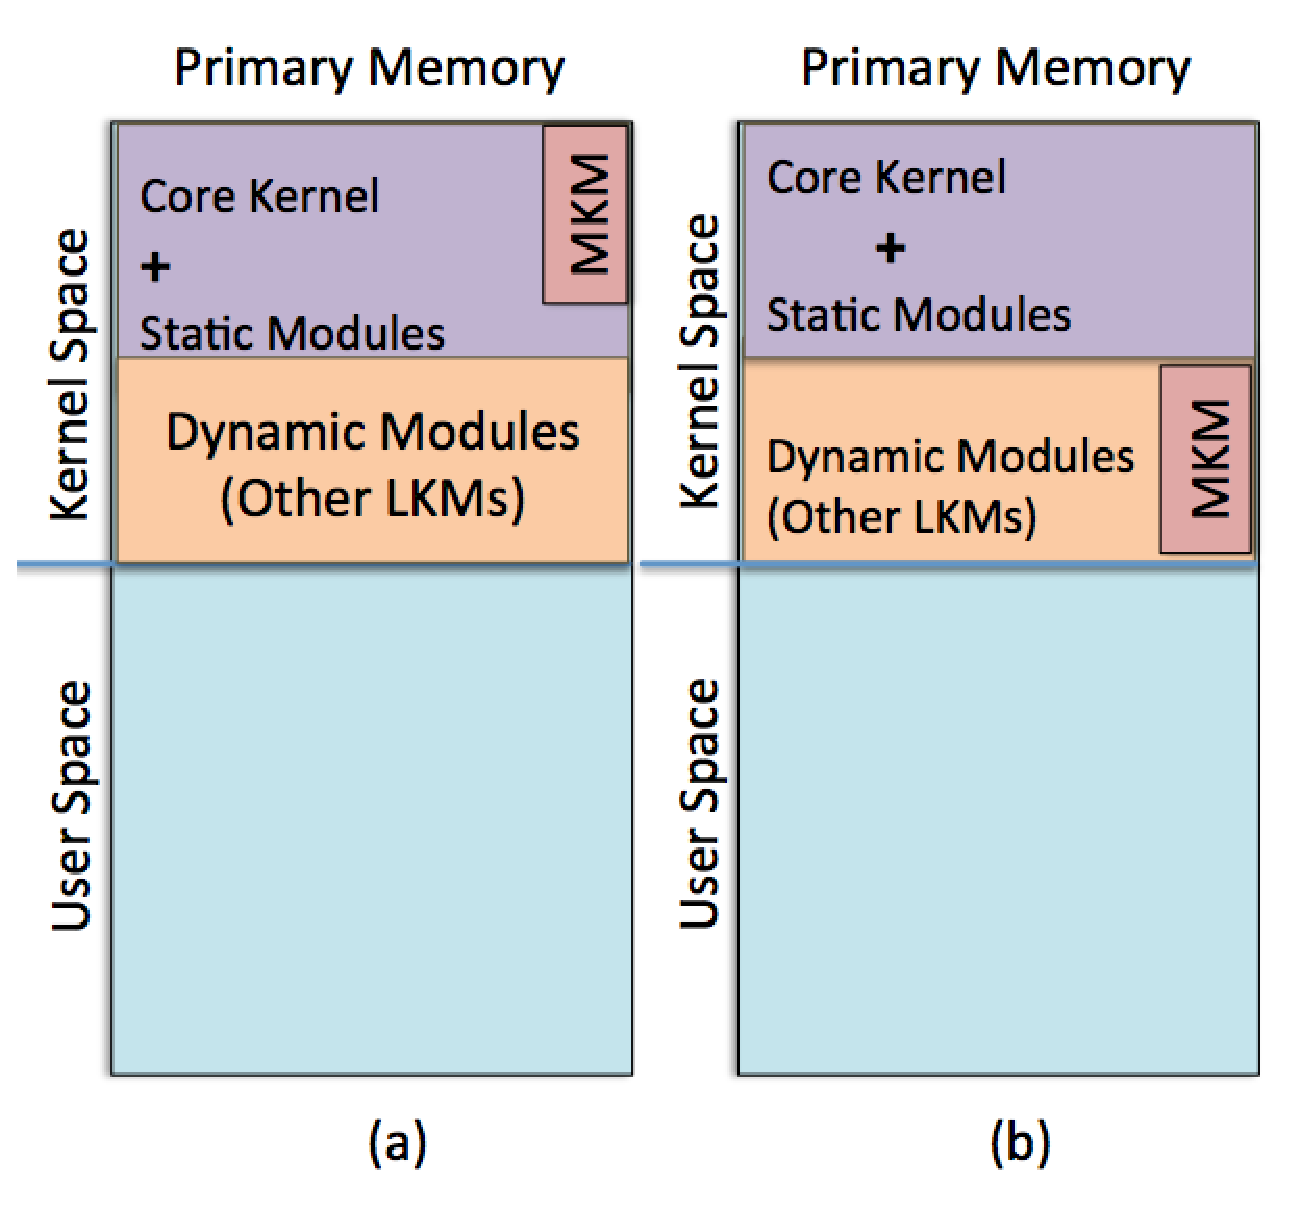
\includegraphics[scale=0.2]{figures/CyFT-MKM.eps}
%\caption{•}
%\end{figure}
\subsubsection{Metrics for Modbus Traffic Analysis Approach}
We propose using the following metrics for validating the proposed KRAFT toolkit's performance under the modbus traffic analysis approach. While numerous metrics exist and provide robust validation, below are the metrics we specifically use for establishing baseline traffic pattern against which KRAFT's performance in effective live forensics of the MCS field devices will be measured. These metrics are -- 
\begin{itemize}
\item \textit{average number of packets per unit time}
\item \textit{average request/response packet size per unit time per device type}
\item \textit{average number of ingress/egress connections per device type}
\item \textit{most frequently used and least frequently used function codes accessed per device type}
\item \textit{average number of u-cast, m-cast, b-cast packets per unit time per device type}
\item \textit{average number of errors reported per unit time per field device type}
\item \textit{average number of request/response with non-standard protocols from unusual ports per unit time per device type}
\end{itemize}

\subsubsection{Metrics for Memory Dump Analysis Approach}
We shall use use the following candidate metrics for validating the proposed KRAFT toolkit's performance under the memory dump analysis approach. The below candidate metrics for validation of KRAFT will be used to first establish a baseline traffic pattern against which KRAFT's ability to support effective live forensics of the MCS field devices will be measured. The suggested metrics are as follows  --
 \begin{itemize}
\item Average allocated memory per process
\item Number of DLLs/Library functions in memory
\item Number of AC violations by processes
\item Network IO usage
\item Central Processing Unit (CPU) usage
\item Number of failed processes/operations logged
\item Number of IPC/RPC calls made per unit of time
\end{itemize}

%\begin{table*}
%\begin{tabular}{ll}\toprule
%\textbf{Modbus Sniffing}	&	\textbf{Memory Dump}	\\\toprule
%Number of packets	&	Average allocated memory per process	\\
%Packet size	&	Number of DLLs/Library functions in memory 	\\
%Number of connections	&	Number of AC violations by processes 	\\
%MFU function codes	&	Network IO usage	\\
%Number of u-cast, m-cast, b-cast packets 	&	Central Processing Unit (CPU) usage	\\
%Average number of errors reported 	&	Number of failed processes/operations logged	\\
%Number of non-standard protocols/ports	&	Number of IPC/RPC calls made per unit of time	\\\bottomrule
%\end{tabular}
%\caption{Solution vectors supporting MCS live forensics.}
%\end{table*}

%\begin{figure}\label{fig:mcs-proto-fp}
%\includegraphics[scale=0.25]{figures/modbus-fp.eps}
%\caption{MCS Field-bus protocol fingerprinting engine.}
%\end{figure}
%
%
%\subsection{FSM-based Live Forensics on MCS}
%
%\begin{figure}\label{fig:mcs-oe-fp}
%\includegraphics[scale=0.16]{figures/mcs-fp-engine.eps}
%\caption{MCS Operating Environment fingerprinting engine.}
%\end{figure}

%We have modeled the system states for the target MCS system as a graph with nodes denoting the system states and edges denoting the transitions. We then model the target system by processing continuous stream of network traffic. An alternate model is to model the process memory dump into a graph of relevant states and transitions.
%
%A state machine-based model is well suited for identifying outlier conditions that can transition the system to unknown, unsecured, and unauthorized states. There are numerous language specific open-source tools that can be extended to SCADA MCS live forensics
%
%Potential candidate tools for phase-II prototyping include – PyFSM, TuLiP (python), Java EasyFSM.

Some of the open source memory forensics tools we have explored in this research work include -- \textit{Rekall, Volatility, Bulk Extractor,} and \textit{LiME}.
\begin{table}[!h]
\begin{center}
\begin{tabular}{ll}\toprule
\textbf{Deviation Impetus}	&	\textbf{Potential Target	}\\\toprule
Unusual access requests	&	-- to devices that were never accessed before	\\
	&	-- from devices that have never requested before	\\
	&	-- to secure/restricted resources (system files)	\\\midrule
Unusual commands		&	-- authorized patterns not seen before	\\
	&	-- unauthorized patterns	\\
	&	-- unreasonable rates 	\\\midrule
Unusual packet format	&	-- valid header but not seen before	\\
	&	-- unknown packet header	\\
	&	-- payload size unusual	\\\midrule
Unusual account access	&	-- too many requests	\\
	&	-- too many failed requests	\\
	&	-- requests to unknown accounts	\\
	&	-- Missing regular and expected requests\\\bottomrule
\end{tabular}
\vspace{2mm}
\caption{Indicators of abnormal events -- malicious and system malfunctions.}
\label{tab:deviation}
\end{center}
\end{table}

\section{Model Evaluation}
\subsection{Validation Framework}
This week, we conducted some testing on Rekall?s WinPMem tool to determine how different operational parameters affect the time and storage space it requires to capture memory dumps.  
\begin{table*}[h]
\begin{center}
\begin{tabular}{l l}\toprule
\textbf{Artifact}	&	\textbf{Evidentiary Information}	\\\toprule
Timestamps	&	Process initialization; Process termination	\\\midrule
Usage pattern	&	  Resident memory usage; CPU and IO activity; Disk capacity and usage; Network activity	\\\midrule
Security/Audit logs	&	 Unauthorized login attempts; Unauthorized access attempts	\\\midrule
System logs	&	Crash, Halt; Shutdown, Reboot	\\\midrule
Activity logs	 &	Processes and Process IDs; Executable-Process ID maps; Resource utilization; Process automation	\\\midrule
Kernel logs (e.g., Unix sys call printk())	&	 Modules loaded and unloaded; Emergency messages; Critical errors\\\bottomrule
\end{tabular}
\end{center}
\end{table*}
Our tests included:
\begin{enumerate}
\item Capturing memory dumps of the same system with different amounts of system memory installed, and recording the time and storage overhead for each.  
\item Capturing memory dumps using different file compression options: the snappy algorithm, the zlib algorithm, and no compression.  Although Rekall?s website claims that snappy compression is the fastest option, we found that storing the files in uncompressed form was often slightly faster on the machine we used.  
\item Observing WinPMem's behavior when we try to append a new memory dump to an existing one. This is the default behavior for when the specified output file already exists.
\end{enumerate}
%\begin{table*}[!t]
%\begin{center}
%\begin{tabular}{l l l l}
%\textbf{Port} & \textbf{Service} & \textbf{Vulnerability} & \textbf{Attack Vector} \\\toprule
%21/TCP  & FTP & Transports userID \& passwords in clear text &
%Man-in-the-Middle: sniffing Masquerading\\
%23/TCP & Telnet & Transports everything as plain text & 
%Man-in-the-Middle: sniffing Masquerading\\
%80/TCP & HTTP & Unpatched Web server & 
%Input validation attacks; injections (sql), url/parameter tampering, etc.\\
%xxx/TCP & Proprietary Service on 502/TCP & Buffer \& Heap Overflows & Remote exploitation via injections (shellcode), unvalidated string input, etc.\\\bottomrule
%\end{tabular}
%\caption{IT network vulnerabilities that impact MCS.}
%\end{center}
%\label{tab:it-vul}
%\end{table*}

\subsection{Transmitting memory dumps via Modbus TCP}
From number of bytes (2) in the message length field, we conclude that each Modbus TCP frame can hold a payload up to 65535 bytes in size. Since very few embedded systems with system memory of 64 KB or less are still in use, any implementation of memory dump transmission via Modbus TCP should be designed to accommodate file splitting on the server side and file splicing on the client side. Table 1 shows how different sizes of memory dump would be split for transmission:

\subsubsection{Packet Crafting Module}
We have implemented a custom kernel module that is a packet crafter such that the memory dump can be packaged into into independent data packets and/or embedded into unused bits of data packets exchanged between the field device and the MTU over the course of several request/response messages.

%\begin{table}[!h]
%\begin{center}
%\begin{tabular}{lll}\toprule
%RAM size (KB) 	&	Frames Required w/o Hash	&	Frames Required with hash\\\toprule
%256	&	4	&	4	\\
%512	&	8	&	8	\\
%64000	&	977	&	977	\\
%256000	&	3907	&	3907	\\\bottomrule
%\end{tabular}
%\caption{Overhead associated with shipping back the RTU/PLC memory dump to the MTU.}
%\label{tab:frames-req}
%\end{center}
%\end{table}


%\begin{table*}[!htbp]
%\begin{center}
%\begin{tabular}{lllllll}\toprule
%	&	\textbf{zlib}	&	\textbf{zlib w/ truncation}	&	\textbf{snappy}	&	\textbf{snappy w/ truncation}	&	\textbf{No compression} &	\textbf{No compression w/ truncation}	\\
%\textbf{Total runtime (s)}	&	451.1445138	&	435.1035562	&	329.1414529	&	349.0159306	&	311.5651912	&	309.7229189	\\
%\textbf{Memdump size (B)}	&	5,347,984,723	&	5,440,281,251	&	5,024,617,223	&	5,920,743,621	&	8,564,930,530	&	8,564,930,531	\\
%%\textbf{Size of Memdump (KiB)}	&	5222641.331	&	5312774.659	&	4906852.757	&	5781976.192	&	8364189.971	&	8364189.972	\\
%\textbf{Memdump size(KB)}	&	5347984.723	&	5440281.251	&	5024617.223	&	5920743.621	&	8564930.53	&	8564930.531	\\
%%\textbf{Size of Memdump (MiB)}	&	5100.235675	&	5188.256503	&	4791.848395	&	5646.461125	&	8168.154268	&	8168.154269	\\
%\textbf{Memdump size (MB)}	&	5347.984723	&	5440.281251	&	5024.617223	&	5920.743621	&	8564.93053	&	8564.930531	\\\bottomrule
%\end{tabular}
%\caption{Compression time and size.}
%\label{tab:compression-truncation}
%\end{center}
%\end{table*}


\subsection{Observations}
In item-3 above, we expected winpmem to either append a complete memory dump to the existing one and double its size, or to append a subset of the address space that had changed since the previous dump was captured. Instead, the program returned an error.  We intend to investigate this further.

Rekall has a small but powerful suite of built-in plugins to analyze Windows registry entries.  In this example, we will use them to find and display registry key pairs contained in our memory dump.  With our image file open in Rekall, we begin by calling the hives plugin.

\subsection{Results}\label{sec:results}

\subsection{Secure Memory Dump Transfer to MTU}
Protecting the data against corruption and truncation would require additional measures. Two possibilities exist to alert the client to any errors in data transmission or splicing:

\begin{enumerate}
\item Transmit a single checksum for the entire memory dump, and verify the integrity of the reassembled dump-file at the MTU.This would require very little overhead. The comparison in Table~\ref{tab:frames-req} shows that for several common RAM configurations, packaging a checksum from the Linux command sha256sum with the memory dump requires no extra packets to be sent. Only one checksum of the memory dump file would be necessary because TCP already performs checksum-based verification of each packet. The only concerning aspect of this method is its potential to become too complex, in terms of computation and disk access, to be feasible on an embedded system.
\item Overlap the transmissions such that each fragment is transmitted with a small amount of data
from the previous fragment. This method would decrease the complexity of disk and computational operations, but transmission overhead would increase proportionally to the size of the overlap.
\end{enumerate}


\section{Conclusion and Future Work}\label{sec:conc}

\section{Definitions}
\begin{myDef}
Cyber-Physical Systems are co-engineered interacting networks of physical and computational components that are built from, and depend upon, the seamless integration of computational algorithms and physical components.
\end{myDef}

\begin{myDef}
Control Systems manage, command, direct or regulate the behaviour of other devices or systems ranging from a home  a thermostat controlling a domestic boiler to large industrial control systems which are used for controlling processes or machines.
\end{myDef}

\begin{myDef}
Industrial control system (ICS) is a general term that encompasses several types of control systems and associated instrumentation used in industrial production, including supervisory control and data acquisition (SCADA) systems, distributed control systems (DCS), and other smaller control system configurations such as programmable logic controllers (PLC) often found in the industrial sectors and critical infrastructures.
\end{myDef}


\begin{myDef}
A programmable logic controller (PLC), or programmable controller is an industrial digital computer which has been ruggedised and adapted for the control of manufacturing processes, such as assembly lines, or robotic devices, or any activity that requires high reliability control and ease of programming and process fault diagnosis.
\end{myDef}

\balance
\begin{myDef}
Supervisory control and data acquisition (SCADA) is a control system architecture that uses computers, networked data communications and graphical user interfaces for high-level process supervisory management, but uses other peripheral devices such as programmable logic controllers and discrete PID controllers to interface to the process plant or machinery.
\end{myDef}

\begin{myDef}
A remote terminal unit (RTU) is a microprocessor-controlled electronic device that interfaces objects in the physical world to a distributed control system or SCADA (supervisory control and data acquisition) system by transmitting telemetry data to a master system, and by using messages from the master supervisory system to control connected objects.
\end{myDef}

\begin{myDef}
A Distributed Control System (DCS) is a computerised control system for a process or plant, in which autonomous controllers are distributed throughout the system, but there is central operator supervisory control.
\end{myDef}

\begin{myDef}
A loadable kernel module (LKM) is an object file that contains code to extend the running kernel (aka base kerne) of an operating system typically used to add support for new hardware (as device drivers) and/or filesystems, or for adding system calls to provide additional functionality.
\end{myDef}

\begin{myDef}
Advanced RISC Machine (ARM) is a family of reduced instruction set computing (RISC) architectures for computer processors, configured for various environments. ARM has reduces costs, heat and power use making it highly desirable for embedded systems in SCADA-MCS environment.
\end{myDef}

\bibliographystyle{plain}
    \bibliography{scada-live-forensics.bib}
\end{document}


